%%%%%%%%%%%%%%%%%  Debut du fichier Latex  %%%%%%%%%%%%%%%%%%%%%%%%%%%%%%
\documentclass[a4paper,12pt,onecolumn]{article}

%%% Pour un texte en francais

%%\usepackage[applemac]{inputenc}
%\usepackage[francais]{babel}
	         % encodage des lettres accentuees
\usepackage[T1]{fontenc}
\usepackage[utf8]{inputenc}          % encodage des lettres accentuees
%\usepackage{graphicx}
%%\usepackage{graphicx} \def\BIB{}
\usepackage[paper=a4paper,textwidth=140mm,left=2.1cm,right=2.1cm,top=2.1cm,bottom=2.1cm]{geometry}
\usepackage{multicol}
\usepackage{graphicx,wrapfig,lipsum} \def\BIB{}
\usepackage[pdftex]{hyperref}
\usepackage[round]{natbib}
\usepackage{perpage} %the perpage package
\MakePerPage{footnote} %the perpage package command
\hypersetup{
    colorlinks,%
    citecolor=black,%
    filecolor=black,%
    linkcolor=black,%
    urlcolor=blue     % can put red here to visualize the links
}
\usepackage{url}

\DeclareUnicodeCharacter{00A0}{ }

%%% Quelques raccourcis pour la mise en page
\newcommand{\remarque}[1]{{\small \it #1}}
\newcommand{\rubrique}{\bigskip \noindent $\bullet$ }

\newcommand{\ignore}[1]{}

\pagenumbering{gobble}

%\bibliographystyle{abbrvnat}
%\setcitestyle{authoryear,open={((},close={))}}

%\renewcommand{\thefootnote}{\roman{footnote}}

% -------------------------------------------------
\newcommand{\horrule}[1]{\rule{\linewidth}{#1}} % Create horizontal rule command with 1 argument of height

\title{	
\vspace*{-2cm}
\normalfont \tiny 
%\textsc{Paris Diderot} \\ [25pt] % Your university, school and/or department name(s)
\horrule{0.5pt} \\[0.4cm] % Thin top horizontal rule
\huge Expos\'e \\ % The assignment title
\horrule{2pt} \\[0.5cm] % Thick bottom horizontal rule
}
\author{E{\sc l mellah} Ileyk} % Your name
\date{\tiny \normalsize 16 Octobre 2017}
%\date{\tiny \normalsize\today} % Today's date or a custom date
% -------------------------------------------------

%\makeatletter
%\def\@xfootnote[#1]{%
%  \protected@xdef\@thefnmark{#1}%
%  \@footnotemark\@footnotetext}
%\makeatother

\begin{document}

\bibpunct{[}{]}{;}{n}{,}{,}

%%%%%%%%%%%%%%%%%%%%%%%%%  PREMIERE PAGE %%%%%%%%%%%%%%%%%%%%%%%%%%%%%%
%%% DANS CETTE PAGE, ON REMPLACE LES INDICATIONS ENTRE CROCHETS [...]
%%% PAR LES INFORMATIONS DEMANDEES
%%%%%%%%%%%%%%%%%%%%%%%%%%%%%%%%%%%%%%%%%%%%%%%%%%%%%%%%%%%%%%%%%%%%%%%

\maketitle
\thispagestyle{empty}

\indent Après 3 années au laboratoire AstroParticule et Cosmologie de l'Université Paris 7 sous la direction de \href{http://www.apc.univ-paris7.fr/~fcasse/}{Fabien Casse} et d'\href{http://www.apc.univ-paris7.fr/APC_CS/en/users/goldwurm}{Andrea Goldwurm}, j'ai soutenu ma thèse le 7 Septembre 2016. Je mène à présent mes activités de recherche et d'enseignement dans le cadre d'une bourse Pegasus Marie Sk\l odowska-Curie à l'université de Leuven, en Belgique, supervisé par \href{https://perswww.kuleuven.be/~u0016541/}{Rony Keppens}. Avec cette candidature à la qualification, je souhaite pouvoir rendre mon dossier éligible aux postes de ma\^itres de conférences qui pourrait correspondre à mon profil dans les ann\'ees \`a venir.

\section*{Recherche}

\indent \indent Avant de commencer ma thèse en Septembre 2013, je me suis porté volontaire pour prendre part à l'analyse des données Kepler sous la direction du \href{http://web.mit.edu/physics/people/faculty/rappaport_saul.html}{Saul Rappaport} au MIT, entre Septembre 2011 et Juillet 2012. Le satellite Kepler est un instrument dédié à l'observation continue, dans le visible, de quelque 150,000 étoiles. Via la méthode des transits, il a permis l'identification d'un nombre conséquent de nouvelles exoplanètes mais a aussi eu pour objet d'étudier les systèmes binaires d'étoiles. En 2012, j'ai participé à la découverte et à la caractérisation de \href{https://en.wikipedia.org/wiki/Kepler-1520}{Kepler-1520}, la première exoplanète de dimension analogue à Mercure et si proche de son étoile qu'elle est en phase de photo-désintégration (\href{https://arxiv.org/abs/1201.2662v2}{Rappaport et al, 2012}). En 2013, grâce notamment à l'algorithme de sélection et d'analyse des éclipses que j'ai développé pour étudier les binaires à courte période orbitale, nous avons pu identifier plus d'une trentaine de systèmes binaires qui abritent en fait une troisième étoile (\href{http://iopscience.iop.org/article/10.1088/0004-637X/768/1/33/meta}{Rappaport et al, 2013}). L'année suivante, le même outil a contribué à l'étude des exoplanètes les plus proches de leur étoile (\href{http://iopscience.iop.org/article/10.1088/0004-637X/787/1/47/meta}{SanchisOjeda et al, 2014}). Cette expérience de recherche fondatrice a jeté les bases de mon projet scientifique : participer à une meilleure compréhension des étoiles et de leurs vestiges, en intéraction avec leur environnement.\\
\indent Les systèmes binaires X, successeurs turbulents des systèmes binaires d'étoiles, offrent des conditions idéales à l'étude de l'évolution stellaire. Ils sont composés d'une étoile dite "donneuse" en orbite avec un objet compact (étoile à neutron ou trou noir) qui siphonne l'enveloppe de son compagnon. Au fur et à mesure que la matière stellaire se rapproche de l'objet compact, elle s'échauffe jusqu'à atteindre des températures dantesques dans son voisinage immédiat et émettre de copieuses quantités de rayons X. C'est ce phénomène de capture gravitationnelle d'un gas ou d'un plasma par un corps massif que l'on appelle accrétion. Les modalités de ce transfert de masse dans les binaires X sont au c\oe ur de mon activité de recherche. 

\subsection*{Accrétion par vent sur un objet compact}

\indent \indent Dans de nombreux systèmes où l'étoile donneuse est de forte masse (les High Mass X-ray Binaries, ou HMXB), le vent stellaire est le principal vecteur de ce transfert de masse. Le puits gravitationnel de l'objet compact, généralement une étoile à neutron, ne capture qu'une fraction de ce vent dense et hautement supersonique. La structure du flot et le taux d'accrétion de masse (i.e. la masse accrétée par unité de temps) conditionnent les observations. Pour confronter les modèles analytiques esquissés par le passé (\href{http://www.sciencedirect.com/science/article/pii/S1387647304000739}{Edgar 2004}), nous avons recouru avec Fabien Casse à un code parallélisé sur grille, \href{http://amrvac.org/}{\texttt{MPI-AMRVAC}}, dont le rôle est de résoudre numériquement des systèmes d'équations hyperboliques telles que les équations de la (magnéto-)hydrodynamique, dans un contexte newtonien ou relativiste. Le principal obstacle à cette approche réside dans les capacités de calcul disponibles face aux contraintes numériques telles que le pas de temps ou la résolution spatiale. Dans le cas présent, le vent supersonique forme un choc détaché autour de l'accréteur à une échelle considérablement plus importante que celle de l'accréteur lui-même. Pour suivre le flot, de la formation du choc jusqu'au voisinage de l'objet compact (là où les rayons X observés sont émis), il m'a fallu construire une grille sphérique centrée sur l'accréteur et telle que la résolution radiale soit proportionnelle à la distance au centre. Ce genre de grilles auto-similaires permettent à la fois de conserver un rapport d'aspect et une résolution relative uniformes, et de sonder des échelles différentes à peu de frais. Dans \href{https://academic.oup.com/mnras/article-abstract/454/3/2657/1206904/Numerical-simulations-of-axisymmetric?redirectedFrom=fulltext}{El Mellah et Casse (2015)}, nous avons, pour la première fois, mis en évidence une propriété topologique afférente au flot d'accrétion qui avait déjà été prédite analytiquement par \href{http://adsabs.harvard.edu/abs/1997A\%26A...320..342F}{Foglizzo et Ruffert (1996)} : une fois le choc passé, le flot accélère suffisamment pour redevenir supersonique sur une surface, la surface sonique, nécessairement ancrée dans l'accréteur (voir Figure\,\ref{fig:fig3}). 

\begin{figure}
\centering
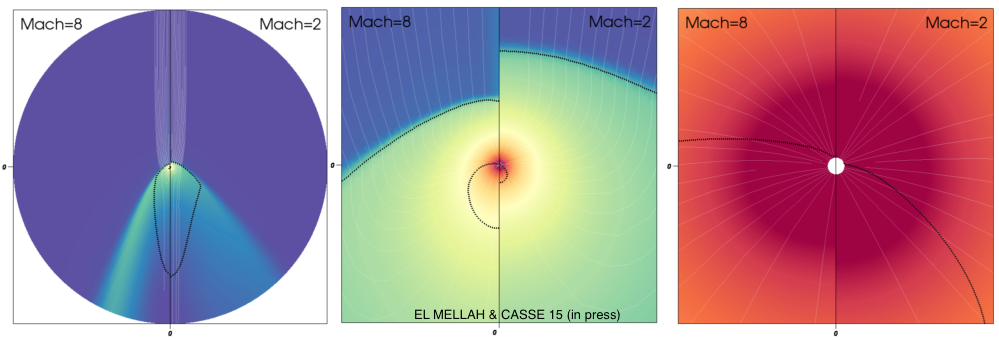
\includegraphics[width=1\columnwidth]{Pictures/FIG3.png}
\caption{Zooms successifs sur la région centrale d'un vent (provenant du haut de l'image) qui est focalisé par le champ gravitationel d'un accréteur central, pour différents nombres de Mach à l'infini. En blanc sont représentées les lignes de champ de vitesse et en noir pointillés, les surfaces Mach-1. L'échelle de couleur, logarithmique, représente la densité de masse.}
\label{fig:fig3}
\end{figure} 

\indent Pour rendre ce modèle numérique plus proche des conditions réelles d'une binaire X, nous avons ensuite évalué l'influence des forces non-inertielles dans le référentiel en co-rotation avec l'étoile et l'objet compact (via le potentiel de Roche). La force de Coriolis par exemple, enroule et cisaille les lignes de champ de vitesse à l'échelle orbitale, si bien que le vent qui parvient au voisinage de l'accréteur n'est plus plan comme dans le cas précédent. Le processus de lancement du vent, basé sur l'absorption résonnante de photons ultra-violet par les orbitales électroniques de métaux partiellement ionisés, a aussi être intégré. Dans \href{https://academic.oup.com/mnras/article-abstract/467/3/2585/2961795/A-numerical-investigation-of-wind-accretion-in?redirectedFrom=fulltext}{El Mellah et Casse (2016)}, j'ai identifié les paramètres déterminants la forme et l'échelle des solutions de déploiement du vent à l'échelle orbitale. Nous avons ensuite exploré l'espace des paramètres afin d'identifier des configurations archétypales. Grâce au couplage entre des propriétés relatives à l'étoile, à son vent, à l'orbite et à l'accrétion, cette approche garantit des résultats cohérents quant à la structure du vent lorsqu'il entre dans le voisinage de l'objet compact.

\indent Les binaires X présentent des niveaux de variabilité spectaculaires, à des échelles et des amplitudes variées. Dans le cas des binaires X Supergéantes (SgXB), une sous-famille des HMXB, la luminosité X peut varier d'un facteur 100 ou plus en quelques heures. L'une des explications avancées porte sur la présence d'inhomogénéités dans le vent des étoiles supergéantes chaudes, notoirement instables (\href{http://adsabs.harvard.edu/doi/10.1086/158342}{Lucy et White 1980}) . Récemment, Sundqvist, Owocki et Puls (soumis) sont parvenus à résoudre ces inhomogénéités dans des simulations 2D d'hydrodynamique radiative, pour des étoiles massives isolées. Afin d'évaluer l'impact de ces inhomogénéités sur la variabilité temporelle du taux d'accrétion de masse (associé à la luminosité X), nous avons d'abord reconstruit une représentation 3D du vent de l'étoile en conservant ses propriétés statistiques (histogrammes, fonction d'auto-corrélation, etc). Ensuite, nous nous sommes servis de ce vent comme condition au bord externe pour l'injecter dans des simulations sur grille centrées sur l'objet compact. La grille, analogue à celle décrite ci-dessus, permet aussi de résoudre les inhomogénéités en augmentant la résolution dans les zones où se manifestent des variations à petite échelle (raffinement adaptatif de grille, AMR). Ces travaux, soumis dans une revue à comité de lecture (El Mellah, Sundqvist et Keppens, 2017), montrent que les inhomogénéités formées dans le vent expliquent la variabilité temporelle lors des phases de basse luminosité mais ne permettent pas, à eux-seuls, de reproduire les sursauts observés.\\

\section*{Enseignement}

\indent \indent Ma première expérience d'enseignement s'est faite dans le cadre de mes études à l'ENS de Cachan. J'ai choisi de réaliser un stage pédagogique au lyc\'ee Gustave Eiffel (94) pour y suivre Vincent Mayer, enseignant en Physique, et découvrir in situ les méthodes d'enseignement dans le secondaire. Pendant ce stage, j'ai donné plusieurs cours à des élèves de Seconde et Terminale S, encadré des travaux pratiques d'optique géométrique et écrit des sujets d'examen. C'est notamment cette expérience enrichissante qui m'a motivé à préparer l'Agrégation en Sciences Physiques l'année suivante. La diversité des sujets abordés pendant cette année, ainsi que la nécessité de se les réapproprier pour pouvoir les restituer en un cours construit, ont considérablement renforcé ma culture en Physique générale. 
\indent Après avoir été re\c cu second à l'Agrégation en 2011, j'ai mis à profit ce bagage en réalisant un monitorat pendant mes 3 années de thèse à l'Université Paris 7 Diderot.

\indent La première année, ma mission d'enseignement s'est déroulée pour moitié (32h TD) en Première Année Commune aux Etudes de Santé (PACES) sous la direction d'Isabelle Grenier à l'hôpital Lariboisière, de Septembre à Octobre 2013. J'y étais responsable de deux groupes de travaux dirigés d'environ 40 étudiants chacun. Le programme de Physique des concours de PACES portent sur un vaste panel de problèmes, de la mécanique des fluides aux intéractions rayonnement-matière. Rendre abordable et compréhensible des notions aussi diverses et dont la maîtrise sérieuse nécessite des outils mathématiques hors de portée des étudiants en première année a représenté un effort aussi considérable qu'instructif. C'est avec enthousiasme que j'ai échangé avec mes collègues moniteurs et notre encadrante sur le contenu des sujets de travaux dirigés et de leurs corrigés que nous co-rédigions. D'Octobre à Décembre 2013, sur le site de l'Université Paris 7 Diderot, j'encadrais les travaux pratiques associés au cours de Master 1 "Traitement du signal - Signaux déterministes" de Laurent Daudet, à hauteur de 32h TD. Cette fois, l'intérêt pédagogique portait sur la transmission de savoirs plus avancés, tant sur le plan théorique (signaux discrets, analyse de Fourier, convolutions, spectre de puissance, filtrage, etc) que pratique (utilisation du langage Matlab pour analyser les données et illustrer les concepts du cours).

\indent La deuxième année, j'ai choisi de m'orienter vers un autre type d'enseignement. Je souhaitais m'adresser à des étudiants tout juste sortis du secondaire mais susceptibles de poursuivre en Physique jusqu'à un niveau M2 voire doctorat. J'ai donc demandé à rejoindre l'équipe de Cécile Roucelle à l'Université Paris 7 Diderot où j'ai encadré les travaux dirigés en Mécanique du point au niveau L1. Durant les 128h TD qui m'ont été assignées en deuxième et troisième année de thèse, j'ai eu le plaisir non seulement de participer à la rédaction des sujets d'exercice mais surtout à former les étudiants aux spécificités du raisonnement physique. A mon sens, la première année d'études supérieures représente un moment charnière dans le cursus des étudiants et requiert donc un encadrement étroit et exigeant. C'est à ce moment que les étudiants prennent pleinement conscience de l'ampleur de la tâche s'ils souhaitent mener à bien des études en Physique et seul un engagement total de l'équipe pédagogique peut leur apporter la motivation nécessaire. Par la suite, les étudiants se saisissent d'une autonomie qu'un manque de discipline personnelle en première année rendrait définitivement hors de portée.

\indent A l'université de Leuven, j'ai encadré des projets scientifiques de M1/M2 dans l'unité d'enseignement "Computational Methods for Astrophysical Applications" dirigée par Rony Keppens ($\sim$60h TD au cours de ma première année de postdoctorat). Poursuivre mon travail de recherche tout en restant en contact avec les étudiants est une chance qui m'a permis de replacer mes travaux et les outils numériques que j'utilise au quotidien dans une perspective plus didactique. L'organisation logistique de l'enseignement, en mettant en place un réseau de machines virtuelles accessibles aux étudiants, a aussi été une composante importante, à garder à l'esprit lorsque l'on souhaite intégrer la dimension numérique à l'enseignement.

\indent Enfin, durant mon année de Master 2, j'ai rejoint l'équipe enseignante des Cours Thalès qui propose aux étudiants dans l'enseignement supérieur des cours particuliers. 

\section*{Organisation et communication}

\indent \indent Afin de tisser des liens forts entre jeunes chercheurs, la Société Fran\c caise de Physique a initié en 2013, sous l'égide de Samuel Guibal (Paris 7), un évènement annuel intitulé les \href{http://rjp.sfp-paris.fr/index2015.html}{Rencontres Jeunes Physiciens (RJP)}. En deuxième année de thèse, je me suis engagé au sein du comité d'organisation des RJP en tant que community manager. Mon rôle a été d'assurer aux Rencontres une visibilité médiatique maximum, tant sur les réseaux sociaux qu'à travers sa principale vitrine, son site Web. Pour garantir la pérennité des RJP, j'ai aussi procédé, avec l'aide du personnel du Conservatoire National des Arts et Métiers où se déroulait l'évènement, à la captation audio et vidéo des interventions orales qui rythmaient la journée, ainsi qu'à leur diffusion. L'évènement, qui a rassemblé quelque 200 doctorants et post-doctorants d'Ile-de-France, a reçu le soutien de nombreuses universités, écoles doctorales et institutions. Pendant ma thèse, j'ai aussi publié une \href{http://homes.esat.kuleuven.be/~ileyk//index.html}{page personnelle} à même de rendre compte de mes travaux au sein de la communauté scientifique.

\indent Parce que l'activité scientifique nécessite aussi d'être connecté au reste de la société, j'ai animé un atelier sur la notion de potentiel en mécanique à destination d'élèves de lycée en Octobre 2016, à l'occasion de la Fête de la Science. Pour ce faire, j'ai mis à profit des outils intéractifs tels que des maquettes de potentiels de Roche que j'ai pu imprimées en 3D grâce à un financement DIM ACAV (Domaine d'Intérêt Majeur en Astrophysique et Conditions d'Apparition de la Vie). J'ai aussi produit une \href{http://demonstrations.wolfram.com/TrajectoryOfATestMassInARochePotential/}{application intéractive en ligne} qui permette d'appréhender empiriquement la notion de potentiel lorsqu'elle est utilisée conjointement avec la maquette suscitée. Plus récemment, j'ai participé à une \href{https://www.mixcloud.com/faconde/faconde-s2e01-vulgarisation/}{émission radiophonique} pour discuter de la communication scientifique et promouvoir sa composante sensible et esthétique, par opposition à la transmission mécanique de résultats scientifiques formatés qui désenchante et, in fine, suscite un relativisme généralisé au sein de la population.

%\newpage
%
%\begingroup
%\raggedright
%\sloppy
%%\newgeometry{left=2cm,right=2cm,top=2.5cm,bottom=2.5cm}
%\setlength{\bibsep}{5pt}
%\small
%\bibliographystyle{plainnat}
%\bibliography{qualif_MdC}
%\endgroup

\end{document}
%%%%%%%%%%%%%%%%%  Fin du fichier Latex  %%%%%%%%%%%%%%%%%%%%%%%%%%%%%%

